\section{Introduction}
\label{sec:intro}
Picture this scenario in life: You 
switch to a new channel on TV, where two persons talking to each other 
caught your attention. You probably wonder, by human nature, 
who these two person are and what is their relationship. This is not too hard
for you, if you listen into the conversation for a while. 
%At first their words don’t make sense to you, so you search the tv series’ 
%title, identify the actors by their photos, read about the identities of 
%and the relationship between these two characters, and finally start to 
%comprehend their words and enjoy the show. Or, you watch for a longer time 
%and gradually find out on your own.\textcolor{red}{(better have a concrete example instead)}
The dialogue content and the language used therein are mutually correlated
with the social relationship between the speakers~\cite{flover}. 
On the other hand, study \cite{mind-reading} finds that when children talk to 
another person, their understanding of the counterpart depends on nature of 
their relationship to the speaker (in that experiment, 3 kinds of 
relationships are involved: mother, siblings, and friends). 
Thus the ability to infer relationship from dialogues and understand
spoken language according to various relationships is an instinctive and 
indispensible part of human cognitive process. In this paper, we explore 
how we humans do this, and whether we can enable machines to do the same.

To study this problem, we first create a dataset of 6307 
dyadic dialogue sessions (averaging 7.72 turns per session) from movies scripts
, each with a fine-grained label about the speakers relationship. 
Relationships are classified into 13 categories, which can be translated 
to coarser-grained taxomonies by combining related categories. 
\figref{fig:instinct} shows a dialogue example from our dataset. 
The construction of and statistics about this dataset will be 
described in \secref{sec:data}. 
To the best of our knowledge, this is currently the only public 
multi-scenario dialogue dataset labelled with personal relationships. 

In preliminary tests conducted by human volunteers, we find that 
the 13-category classification task is hard
($39\%$ average accuracy) even for human beings due to the limited length 
of each dialogue session. We hence focus on a relaxed, family/workplace binary 
classification problem in this paper, which has 3114 samples in our dataset 
and \textbf{81.68\% human accuracy}. 

\begin{figure}[t!]
	\centering
	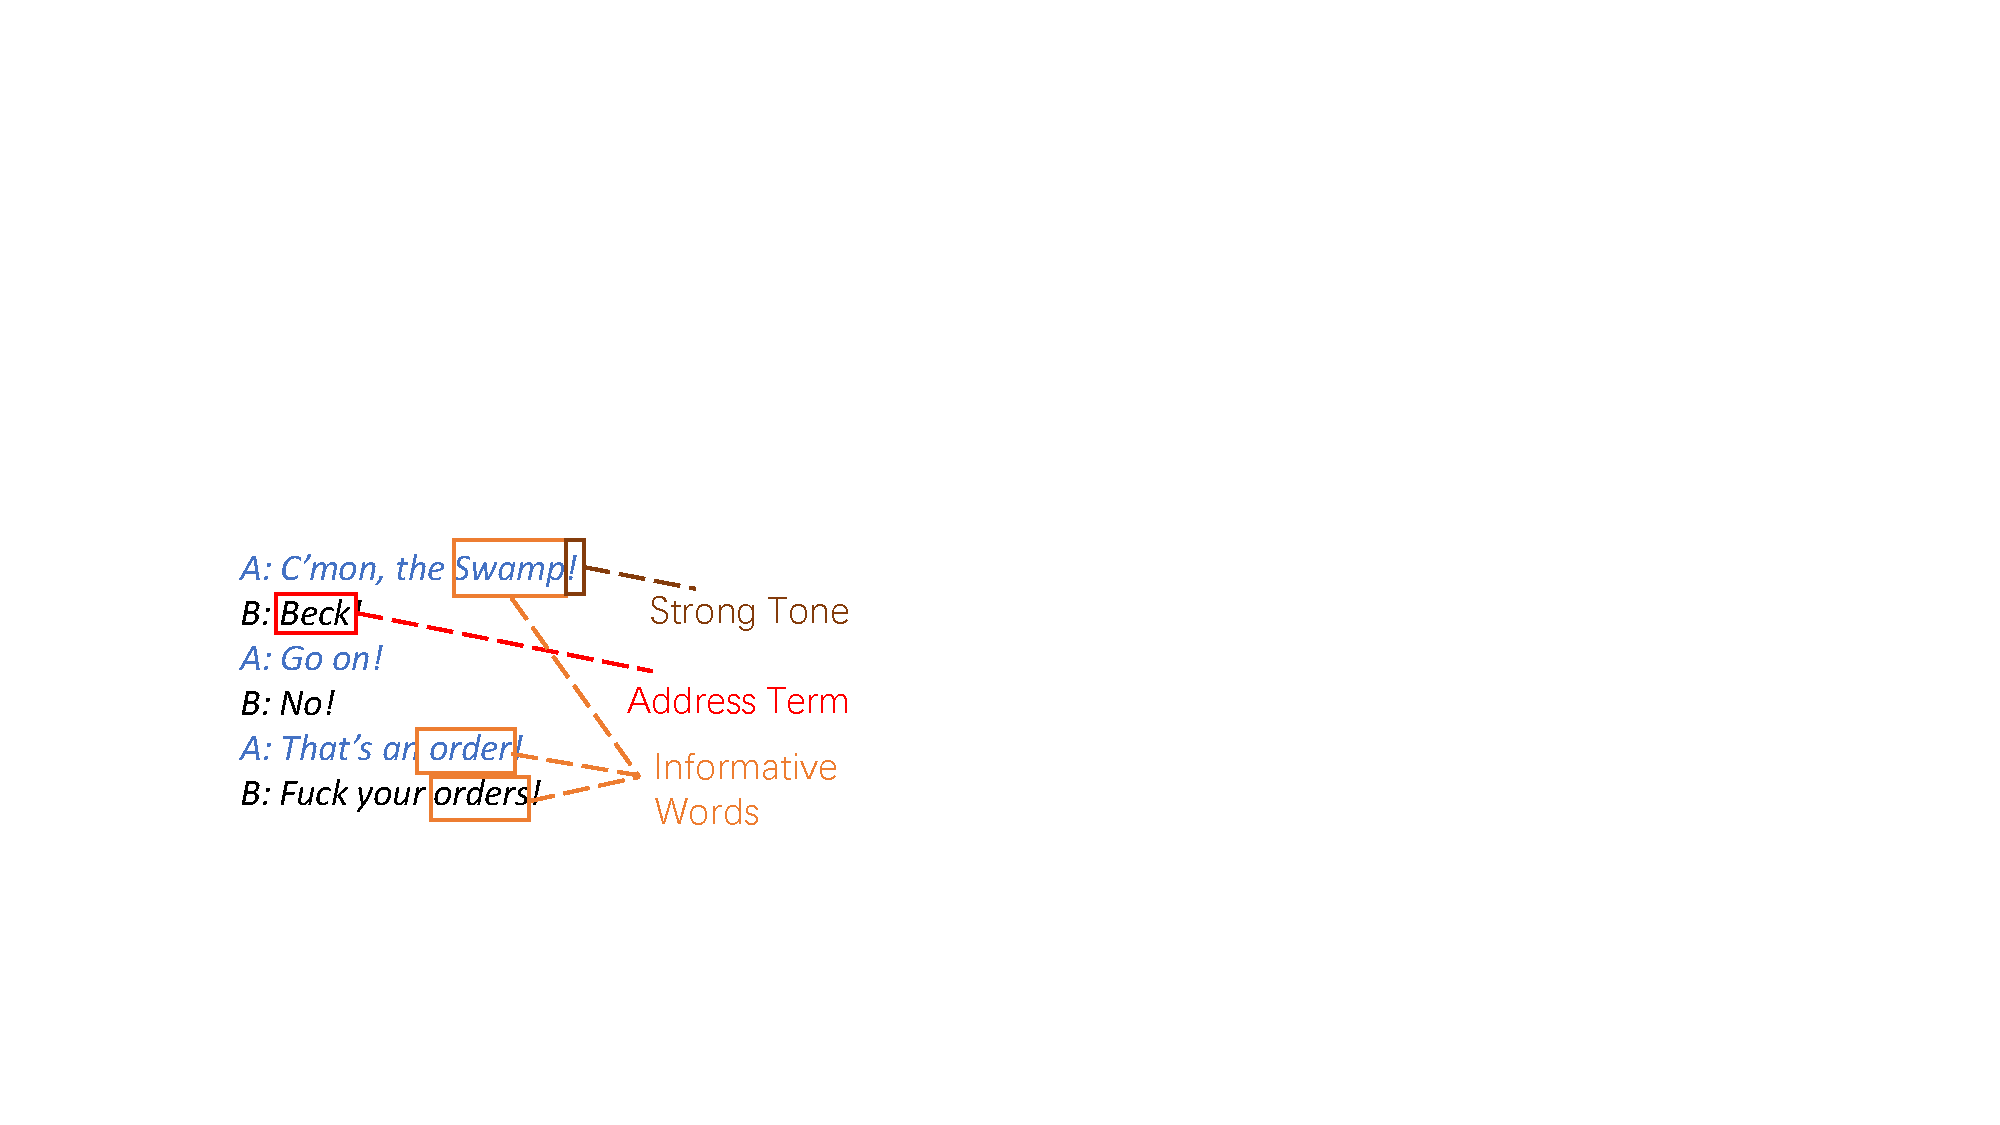
\includegraphics[width=0.85\columnwidth]{instinct.pdf}
	\caption{A sample \textbf{workplace} dialogue and parts that are reported as informative by human testers.}
	\label{fig:instinct}
\end{figure}
To the best of our knowledge, there is no previous research on the same task, 
while related work exists in relationship mining. 
Previous work have focused on
identifying connection or measuring familarity by counting 
how many times two people are involved in one action~\cite{relation-act} 
or conversation~\cite{relation-conver}. 
Chaturvedi et al. have done much work in identifying relationships 
from books or narrative summary~\cite{rel-mining-1,rel-mining-2,rel-mining-3}. 
They either model relationships simply as a bipolar variable (friend/enemy), or use unsupervised ways to cluster those with similar patterns. However, they all use narrative texts such as plot summary in their work, where relationship information is more explicitly stated. Different from all above, in this paper we focus on linguistic cues in dialogues that are indicative of relationships.

Since this can be viewed as a text classification problem, our first attempt is
neural network approaches which boast state-of-the-art performance on many text classification tasks in recent years. These
include character-level convolutional networks (CNN)~\cite{cnn}, 
recurrent neural networks based on long short-term memory (LSTM)~\cite{lstm} 
and hierarchical attention networks~\cite{hierarchy}. 
None of these complex models performs well (see \secref{sec:eval}) due to the limited size and 
heterogenuity of the dataset. 
%given the wide range of topics, intentions and attitudes that can appear in movie dialogues, our dataset doesn't provide enough samples for the networks to learn clear, stable rules. \textcolor{red}{[could add classic relationship extraction methods]} 
To this end, we believe the solution to this {\em small data} learning problem
lies in manually crafted features particular designed to minic human's 
inference process. 

\citeauthor{flover}~\shortcite{flover} states in a previous study that rules of 
language at the phonemic and morphophonemic levels should be highly stable across 
relationship types, but the lexical, syntactic, and pragmatic levels of language are 
strongly affected by social context. To get a more concrete idea about the 
context-variant parts, we pose this task to human volunteers and 
survey them about 
what they find helpful in their inference process. 
The survey shows that there are numerous factors. 
Take the dialogue session in \figref{fig:instinct} as an example.
Constant use of exclamation points indicate strong tone, 
which makes them sound like arguing.
From the nickname address term ``Beck'' and the phrase ``come on'', 
we infer the two speakers are familiar with each other. 
The mention of ``order'' is very indicative of a work relationship with 
disparity in ranking... 
Generally speaking, both informational indicators and sentimental 
hints are taken into acconut.
% \KZ{I think you are being too detailed here. Some of the followings can be
%moved to approach. You use the figure to illustrate 1) how difficult the problem
%is and 2) some indicative features. But you can talk rather 
%superficially here.} %Basically, an informative address term such as "dad", "sir" will immediately make things clear. There are also certain topics, or keywords, that provide much certainty. For example, two people talking about kitchen utensils and dinner are likely family members, and if we find "authentication", "report" and "office" in the dialogue, a work place picture emerges in our minds. Without those informative words, we observe tones, which can be reflected by punctuatiosn, modals, sentence types and so on. A higher level of comprehension is based on common sense. Take the sample in figure \ref{fig:instinct}: by asking "Will your father like me", we can infer that the speaker is about to meet his/her lover's family members and seems worried. 
% Achieving such kind of common sense inference ability is actually a very challenging task for artificial intelligence researchers.

In this paper, we \textbf{define multiple features corresponding to 
those observations, and provide a set of tools to extract and vectorize them 
automatically}, such as an address term identification tool, 
which achieves a 92.15\% match with human labellers on 
917 sentences, and a sentence type recognizer which is able to 
identify certain linguistic patterns such as disjunctive questions, 
imperatives and entrainment. We feed our new features along with 
other previously studied features in related field,  
such as Linguistic Inquiry and Word Counts (LIWC)~\cite{liwc}, into 
Logistic Regression classifier, and achieve very reasonable accuracies on 
the binary classification problem. 
What's more, by analyzing the results, we have some interesting 
findings, e.g., male pronouns (``he, his, him'') show up significantly more 
in workplace conversations, while the prevalence of female pronouns 
hints a family relationship. More about our experiments, features and 
results are introduced in \secref{sec:eval}. 
Besides the interesting nature of this problem, 
we also hope our dataset and methods can help with further research 
in this field. We have a preliminary discussion about possible 
applications and future work in \secref{sec:conclusion}.

In sum, this paper makes the following contributions:
\begin{itemize}
\item we create the first cross-domain dialogue-to-relationship dataset 
for future study (\secref{sec:data});
\item we propose a simple but effective framework to computationally predict
personal relationships from short dialogues (\secref{sec:method});
\item experiments show that our proposed features, together with the 
classification model achieve $78.49\%$ accuracy on the binary classification
problem, very close to the human performance of $81.68\%$ (\secref{sec:eval});
\item we discover several interesting signals, 
such as usage of prepositions, that are not consciously noticed 
by humans but very helpful in classification (\secref{sec:method}).
\end{itemize}

